\documentclass[9pt,a4paper,twocolumn,twoside]{tau-class/tau}
\usepackage[spanish,es-nodecimaldot,es-noindentfirst]{babel}
\usepackage{booktabs}
\usepackage{longtable}
\usepackage{hyperref}

\graphicspath{{figures/pizzeria-loja/}}

\doctype{Reporte de competencia}
\title{Investigacion competitiva: pizzeria en Loja (Ecuador)}

\author[a,1]{Equipo de Analitica Oderbiz}
\affil[a]{Unidad de Inteligencia Comercial}

\dates{Compilado el \today}
\docinfo{Documento elaborado a partir de fuentes publicas oficiales (sitios de marca, perfiles de negocio en redes y fichas de Google Maps). Toda inferencia esta etiquetada como \texttt{inferencia}. Las capturas se obtuvieron el 4 de mayo de 2026.}
\footinfo{Reporte Oderbiz}
\theday{\today}
\organization{Oderbiz}
\leadauthor{Equipo Oderbiz}

\begin{abstract}
Se analizaron tres competidores confirmados por el cliente en el segmento de pizza en Loja: Papa John's (cadena), D'One Pizzeria (local) y Funghi Pizzeria (restaurante italiano con fuerte foco en pizza) (\texttt{observado}). Papa John's concentra presencia de marca nacional con pedido en linea y telefono, volumen de opiniones en Google Maps muy superior al resto y rango de precio por persona informado por usuarios en Maps (\texttt{observado}). D'One muestra comunicacion promocional activa en Facebook con precios en publicaciones y volumen de seguidores moderado (\texttt{observado}). Funghi combina restaurante con canal digital principal en Facebook y mayor base de seguidores entre los dos locales independientes (\texttt{observado}). No se logro evidencia visual de Instagram en esta corrida (\texttt{observado}). Oportunidad clave: diferenciar propuesta local frente a cadena (historia, ingredientes lojanos, combos barrio) y ordenar precios y horarios de forma estable fuera de solo redes sociales (\texttt{inferencia}).
\end{abstract}

\keywords{pizzeria, Loja, Ecuador, competencia, Meta, Google Maps}

\begin{document}
\maketitle
\thispagestyle{firststyle}

\section{Contexto y alcance}

\textbf{Industria:} pizzeria (\texttt{observado}, declarado por el cliente).

\textbf{Ciudad:} Loja, Ecuador (\texttt{observado}).

\textbf{Competidores incluidos:} Papa John's Loja; D'One Pizzeria; Funghi Pizzeria (\texttt{observado}, confirmados por el cliente en la misma sesion).

\section{Matriz comparativa}

\begin{table*}[t]
  \centering
  \small
  \begin{tabular}{@{}p{3.2cm}p{3.8cm}p{3.8cm}p{3.8cm}@{}}
    \toprule
    & \textbf{Papa John's} & \textbf{D'One} & \textbf{Funghi} \\
    \midrule
    Tipo & Cadena de pizza, delivery y local (\texttt{observado}) & Pizza para llevar, local (\texttt{observado}) & Restaurante italiano (\texttt{observado}) \\
    Web propia marca & \href{https://papajohns.com.ec/loja/}{papajohns.com.ec/loja} (\texttt{observado}) & Perfil Facebook como canal principal (\texttt{observado}) & Enlace a Facebook desde Maps (\texttt{observado}) \\
    Facebook & No analizado en profundidad en esta corrida (\texttt{observado}) & \href{https://www.facebook.com/donepizzas/}{facebook.com/donepizzas} (\texttt{observado}) & \href{https://www.facebook.com/funghipizza/}{facebook.com/funghipizza} (\texttt{observado}) \\
    Instagram & Perfil nacional referido \texttt{@papajohnsec}; pagina no cargo en el navegador usado (\texttt{observado}) & No se identifico URL oficial de Instagram en esta corrida (\texttt{observado}) & No se identifico URL oficial de Instagram en esta corrida (\texttt{observado}) \\
    Google Maps (ficha) & \href{https://www.google.com/maps/place/Papa+Johns+Pizza/@-3.9947043,-79.1994322,17z/data=!3m1!4b1!4m6!3m5!1s0x91cb47ca4ea989ff:0xa356ebcb687e0b27!8m2!3d-3.9947043!4d-79.1994322!16s\%2Fg\%2F11qgchhq_6}{Papa Johns Pizza} (\texttt{observado}) & \href{https://www.google.com/maps/place/D'+One+Pizzer\%C3\%ADa/@-4.0095863,-79.2026892,17z/data=!3m1!4b1!4m6!3m5!1s0x91cb37ec2293cf37:0xc6694bc6bef821ee!8m2!3d-4.0095863!4d-79.2026892!16s\%2Fg\%2F11l2x4nmcc}{D' One Pizzeria} (\texttt{observado}) & \href{https://www.google.com/maps/place/FUNGHI+PIZZERIA/@-3.9977592,-79.1982236,17z/data=!3m1!4b1!4m6!3m5!1s0x91cb380076488db5:0x5bb04e7c085c2bb2!8m2!3d-3.9977592!4d-79.1982236!16s\%2Fg\%2F1pp2tlp7p}{FUNGHI PIZZERIA} (\texttt{observado}) \\
    Resenas Maps (conteo mostrado) & 427 opiniones (\texttt{observado}) & 17 opiniones (\texttt{observado}) & 19 opiniones (\texttt{observado}) \\
    Rango precio Maps & USD 5--10 por persona, informado por 53 personas (\texttt{observado}) & USD 5--10 por persona, informado por 9 personas (\texttt{observado}) & No aparecio el mismo indicador en la ficha capturada (\texttt{observado}) \\
    Horario (Maps) & Abierto; cierre 22:00 (\texttt{observado}) & Abierto; cierre 22:00 (\texttt{observado}) & Lun--jue 15:00--23:00; vie--dom 12:00--23:00 (\texttt{observado}) \\
    Telefono (Maps) & 099 562 2233 (\texttt{observado}) & 096 301 0289 (\texttt{observado}) & (07) 257-0344 (\texttt{observado}) \\
    \bottomrule
  \end{tabular}
  \caption{Comparativo resumido (mayo 2026).}
  \label{tab:matriz}
\end{table*}

\section{Papa John's Loja}

\subsection{Propuesta y canales}
Sitio oficial de sucursal con direccion Av.\ Emiliano Ortega y Juan Jose Pena, pedidos en linea y por telefono, correo \texttt{loja@papajohns.com.ec} y telefonos 099 56 222 33 y 022942733 (\texttt{observado}, captura web).

\subsection{Google Maps}
Ficha con categoria pizzeria, enlace a menu en \texttt{papajohns.com.ec}, boton de pedido en linea y volumen de opiniones 427 (\texttt{observado}). Valoracion por estrellas: ver captura; no se transcribio el numero exacto desde el arbol de accesibilidad del navegador (\texttt{observado}).

\subsection{Redes}
El perfil \texttt{@papajohnsec} devolvio error de carga en la sesion automatizada (\texttt{observado}).

\begin{figure}[h]
  \centering
  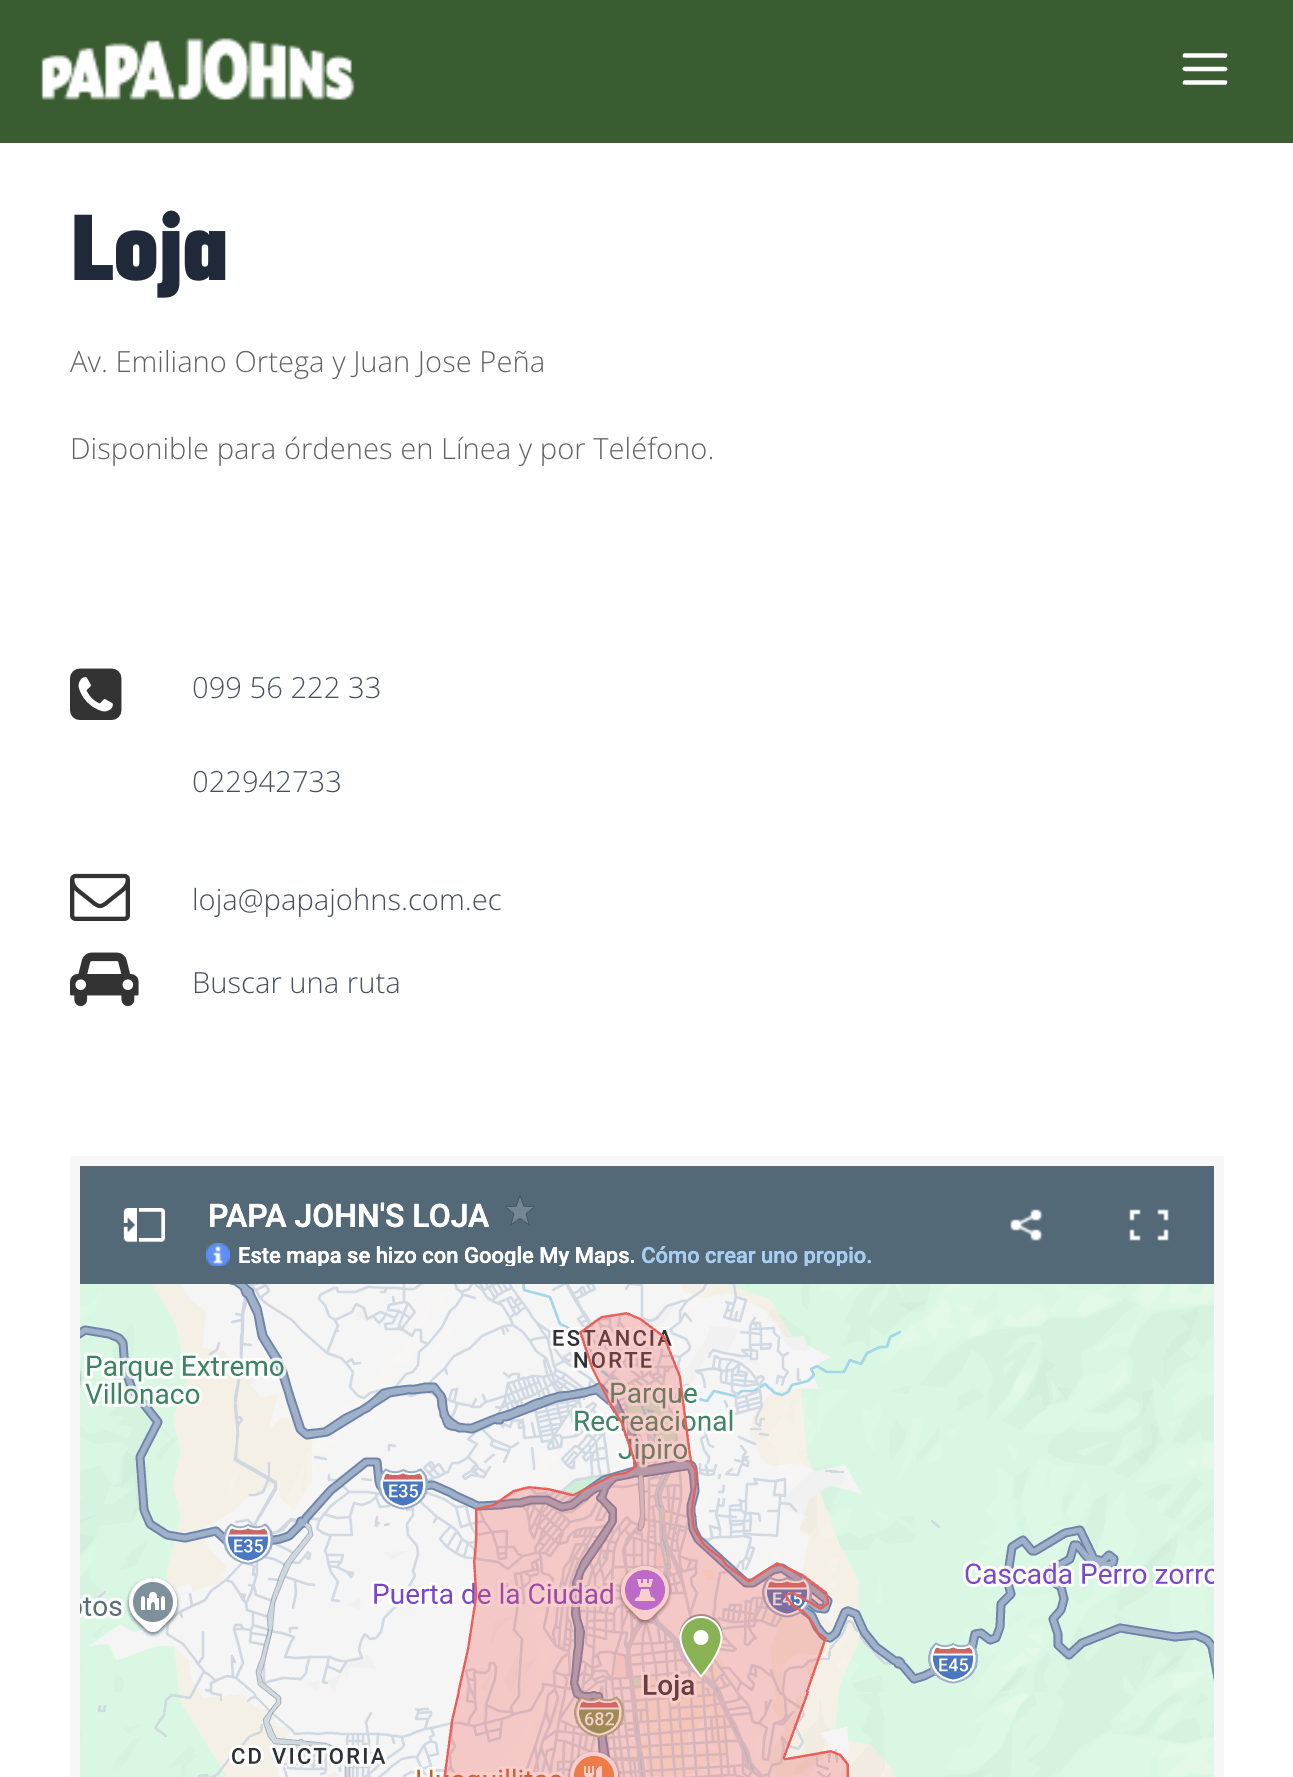
\includegraphics[width=\linewidth]{fig-web-papajohns-loja-20260504-v1.png}
  \caption{Sucursal Loja en sitio oficial Papa John's Ecuador. Origen: \url{https://papajohns.com.ec/loja/}. Fecha: 2026-05-04.}
  \label{fig:pj-web}
\end{figure}

\begin{figure}[h]
  \centering
  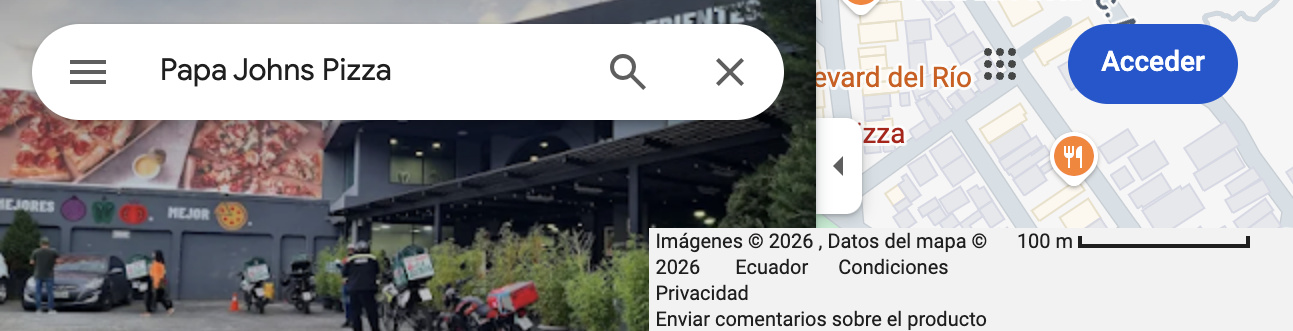
\includegraphics[width=\linewidth]{fig-maps-papajohns-20260504-v1.png}
  \caption{Ficha Google Maps. Origen: busqueda desde \url{https://www.google.com/maps/}. Fecha: 2026-05-04.}
  \label{fig:pj-maps}
\end{figure}

\section{D'One Pizzeria}

\subsection{Facebook}
Perfil de negocio con categoria Pizzeria, direccion en calle 18 de Noviembre y Chile, Loja, texto de recomendacion visible y publicaciones con ofertas (ej.\ mencion a dos pizzas por USD 11,49 en el feed visible) (\texttt{observado}). Seguidores mostrados: 421 (\texttt{observado}).

\subsection{Google Maps}
Categoria \emph{Pizza para llevar}, direccion Chile y C.\ Zapotillo \&{}, Loja, telefono 096 301 0289, enlace a menu externo \texttt{n9.cl}, 17 opiniones, rango USD 5--10 por persona segun informacion de Maps (\texttt{observado}). El campo sitio web apunta a \texttt{lojaecuador.com} (\texttt{observado}); conviene tratarlo como senal secundaria frente a web propia del negocio (\texttt{inferencia}).

\begin{figure}[h]
  \centering
  
\includegraphics[width=\linewidth]{fig-facebook-done-20260504-v1.png}
  \caption{Perfil Facebook D'One. Origen: \url{https://www.facebook.com/donepizzas/}. Fecha: 2026-05-04.}
  \label{fig:done-fb}
\end{figure}

\begin{figure}[h]
  \centering
  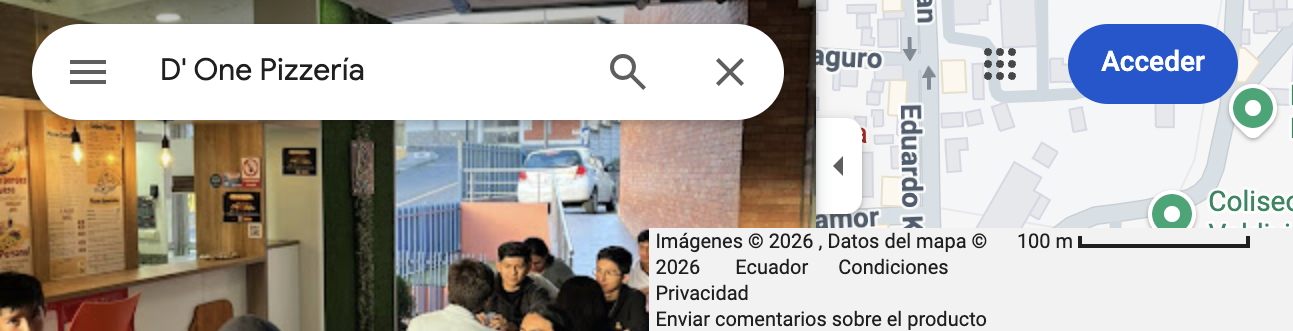
\includegraphics[width=\linewidth]{fig-maps-done-20260504-v1.png}
  \caption{Ficha Google Maps D'One. Origen: \url{https://www.google.com/maps/}. Fecha: 2026-05-04.}
  \label{fig:done-maps}
\end{figure}

\section{Funghi Pizzeria}

\subsection{Facebook}
Nombre comercial \emph{Funghi Pizzeria Restaurante}, direccion Av.\ Universitaria, Celica y Cariemanga, Loja, 1567 seguidores (\texttt{observado}).

\subsection{Google Maps}
Categoria restaurante italiano, direccion 24 de Mayo (codigo Plus 2R22+VPR), telefono (07) 257-0344, 19 opiniones, enlace de sitio web a Facebook (\texttt{observado}). Horarios detallados lun--jue 15:00--23:00 y vie--dom 12:00--23:00 (\texttt{observado}).

\begin{figure}[h]
  \centering
  
\includegraphics[width=\linewidth]{fig-facebook-funghi-20260504-v1.png}
  \caption{Perfil Facebook Funghi. Origen: \url{https://www.facebook.com/funghipizza/}. Fecha: 2026-05-04.}
  \label{fig:funghi-fb}
\end{figure}

\begin{figure}[h]
  \centering
  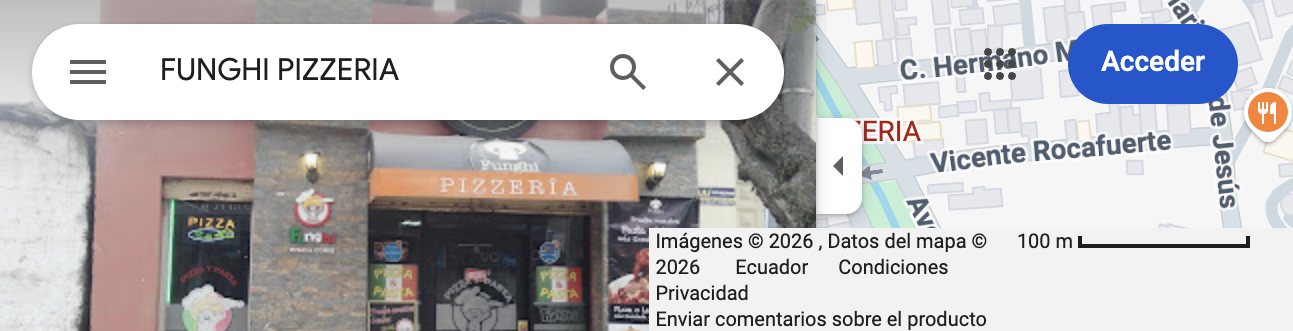
\includegraphics[width=\linewidth]{fig-maps-funghi-20260504-v1.png}
  \caption{Ficha Google Maps Funghi. Origen: \url{https://www.google.com/maps/}. Fecha: 2026-05-04.}
  \label{fig:funghi-maps}
\end{figure}

\section{Diagnostico y oportunidades (\texttt{inferencia})}

\begin{itemize}
  \item \textbf{Presion de marca:} Papa John's combina sitio propio, pedido digital y muchas resenas; compite por confianza de marca y escala (\texttt{inferencia}).
  \item \textbf{Agilidad local:} D'One y Funghi pueden mover ofertas y tono comunitario mas rapido en Facebook (\texttt{inferencia}).
  \item \textbf{Brecha digital:} Ausencia estable de Instagram verificada en esta corrida deja canal abierto para formato video/reels si el mercado lo usa (\texttt{inferencia}).
\end{itemize}

\section{Fuentes y limitaciones}

\subsection{Fuentes}
Sitio \url{https://papajohns.com.ec/loja/}; fichas de Google Maps enlazadas en la tabla; \url{https://www.facebook.com/donepizzas/}; \url{https://www.facebook.com/funghipizza/}; capturas en \texttt{docs/reports/figures/pizzeria-loja/} con nombres \texttt{fig-*-20260504-v1.png} (\texttt{observado}).

\subsection{Limitaciones}
\begin{itemize}
  \item Instagram: error de carga para \texttt{instagram.com/papajohnsec/} en el navegador automatizado; no se capturo feed (\texttt{observado}).
  \item No se revisaron anuncios activos en Meta Ads Library en esta corrida (\texttt{observado}).
  \item Direcciones entre Facebook y Google Maps pueden mostrar redacciones distintas para el mismo negocio; conviene validar en campo (\texttt{inferencia}).
  \item Precios de carta completos no fueron sistematizados; solo indicios (rango Maps, oferta visible en Facebook para D'One) (\texttt{observado}).
\end{itemize}

\end{document}
